\chapter{Introducing Correlations in Larval Trait Parameters}
Larval trait parameters used in the model are considered to be independent of each other while assigning to each individual. This model can be useful to understand distributions of these trait parameters and other life-history traits with development time after few generations of selection in each density regime. It can also give more detailed insight on how larval trait parameters interact with larval density as well as how early eclosing and late eclosing flies are different in these populations.
\section{Distribution of Laral Traits with Development Time}
Simulations are run using the initial conditions for MB, MCU, CCU and MCU populations given in tabel (no.) at all four densities (replicates = 10, generation = 50). Results from these simulations are plotted for larval body size, final feeding rate (at critical size), efficiency, initial feeding rate, critical size and efficiency. Similar to previous simulations, time to reach critical size is taken as a proxy for development time (see fig~\ref{fig:lh_mb_culture} - \ref{fig:lh_lcu_culture}). For each of the above traits, a scatter plot is plotted, where trait value is plotted as an 'x-estimator' of respetive development time (ref). These plots give a clear visualization of mean trait value distribution with development time. Mean trait values towards the right size of the x-axis represent late eclosing flies where as such values towards left side of x-axis represent early eclosing flies.\\\\
In these plots, MB larvae take more to reach critical size compared to MCU, CCU and LCU larvae due to higher critical size, lesser efficiency and initial feeding rate. In MB culture (60 eggs / 6 ml), There is no pattern of body size, efficiency, initial feeding rate and waste tolerance with development time. Since critical size is higher for larvae with higher development time, final feeding rate is also higher in them across all populations (see fig~\ref{fig:lh_mb_culture}). \\\\
In MCU culture (600 eggs / 1.5 ml), results are similar to mean trait value distributions in MB culture except, deacrese in mean body size of late eclosing ones in MCU population. Variation in mean body size is higher for both early and late developing larvae for all populations in this culture (see fig~\ref{fig:lh_mcu_culture}). \\\\
In CCU culture (1200 eggs / 3 ml), mean body size and efficiency stays constant across development time but the variation is very less for late developing larvae. Initial feeding rate is slightly higher with reduced variation for larvae with higher development time. Waste tolerance is higher with a decrease in variraiotn for late developing larvae (see fig~\ref{fig:lh_ccu_culture}). \\\\
In LCU culture (1200 eggs / 6 ml), mean trait values are similar to those in CCU culture except, mean body size, which shows that late developing larvae have similar body size as early ones. This forms a U-shapd mean trait value distribution. For late developing larvae in this culture, initial feeding rate is also lesser and variation in efficiency is higher across all popularions. Mean waste tolerance distribution show late developing larave have higher waste tolerance which is more prominent in MCU and LCU populations (see fig~\ref{fig:lh_lcu_culture}).
\begin{figure}[p]
  \subfloat[Mean body size distribution]{
  \centering
  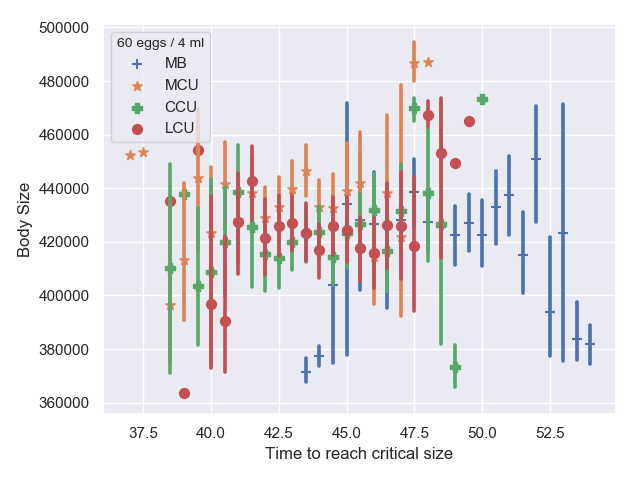
\includegraphics[width=.5\textwidth]{C6/Figs/devt_dist/alive_size_vs_devt_MB}
  }
  \subfloat[Mean final feeding rate distribution]{
  \centering
  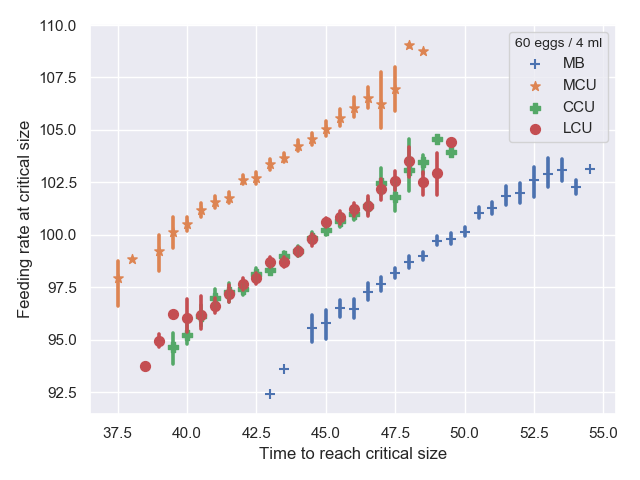
\includegraphics[width=.5\textwidth]{C6/Figs/devt_dist/alive_frt_vs_devt_MB}
  }\\
  \subfloat[Mean efficiency distribution]{
  \centering
  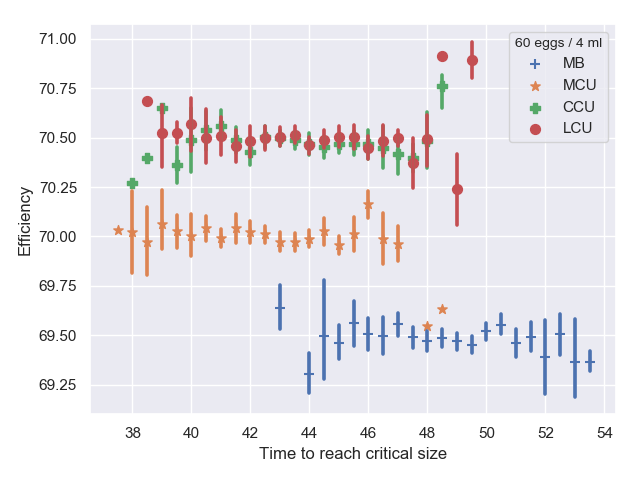
\includegraphics[width=.5\textwidth]{C6/Figs/devt_dist/alive_eff_vs_devt_MB}
  }
  \subfloat[Mean initial feeding rate distribution]{
  \centering
  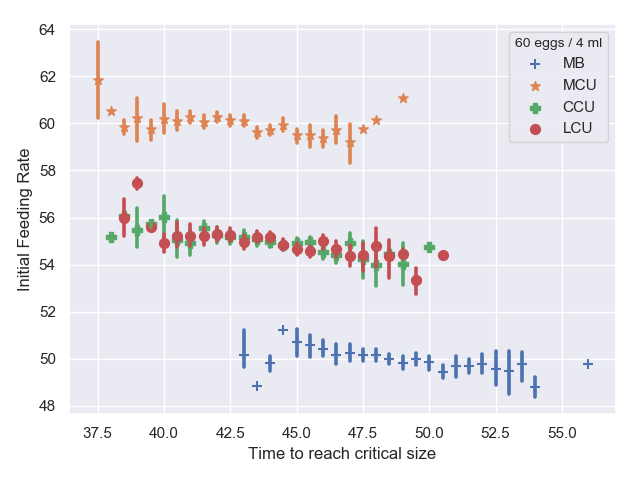
\includegraphics[width=.5\textwidth]{C6/Figs/devt_dist/alive_frc_vs_devt_MB}
  }\\
  \subfloat[Mean critical size distribution]{
  \centering
  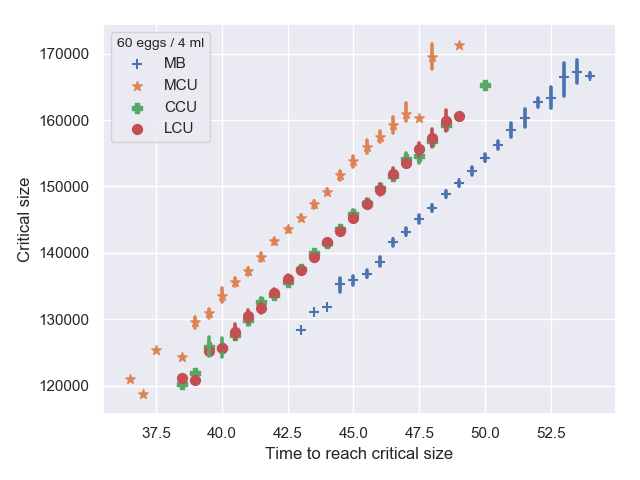
\includegraphics[width=.5\textwidth]{C6/Figs/devt_dist/alive_mc_vs_devt_MB}
  }
  \subfloat[Mean waste tolerance distribution]{
  \centering
  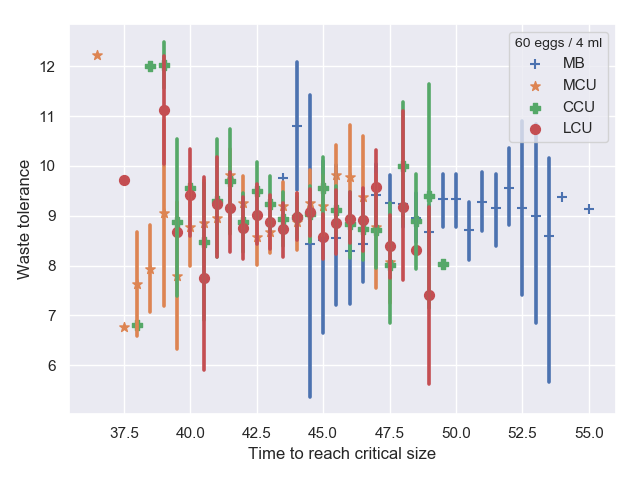
\includegraphics[width=.5\textwidth]{C6/Figs/devt_dist/alive_wt_vs_devt_MB}
  }
  \caption{Mean trait value distribution of MB, MCU, CCU and LCU populations in 60 eggs / 6 ml density at $50^{th}$ generation}
  \label{fig:lh_mb_culture}
\end{figure}
\begin{figure}[p]
  \subfloat[Mean body size distribution]{
  \centering
  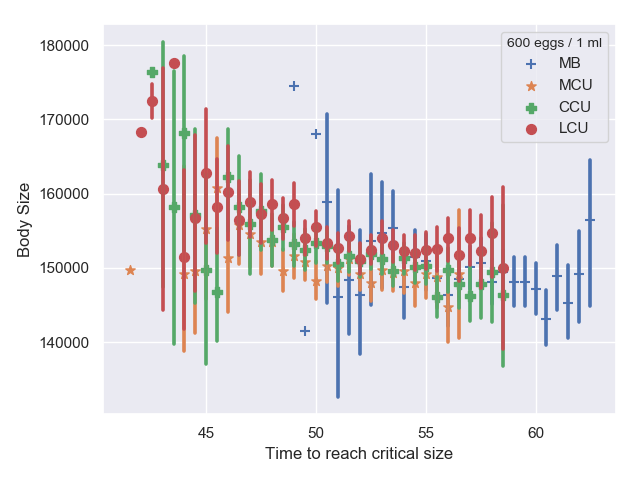
\includegraphics[width=.5\textwidth]{C6/Figs/devt_dist/alive_size_vs_devt_MCU}
  }
  \subfloat[Mean final feeding rate distribution]{
  \centering
  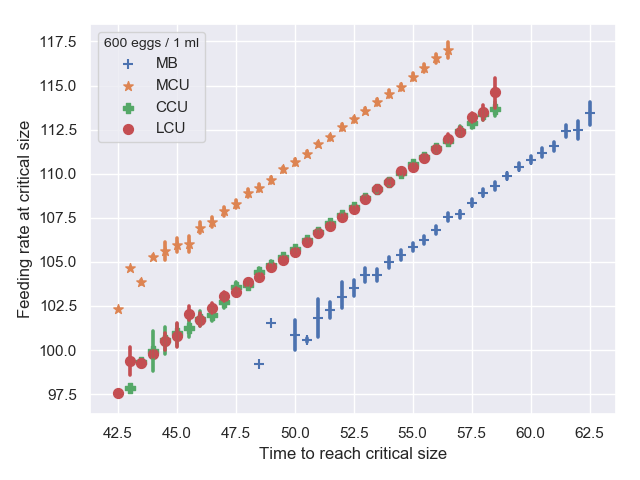
\includegraphics[width=.5\textwidth]{C6/Figs/devt_dist/alive_frt_vs_devt_MCU}
  }\\
  \subfloat[Mean efficiency distribution]{
  \centering
  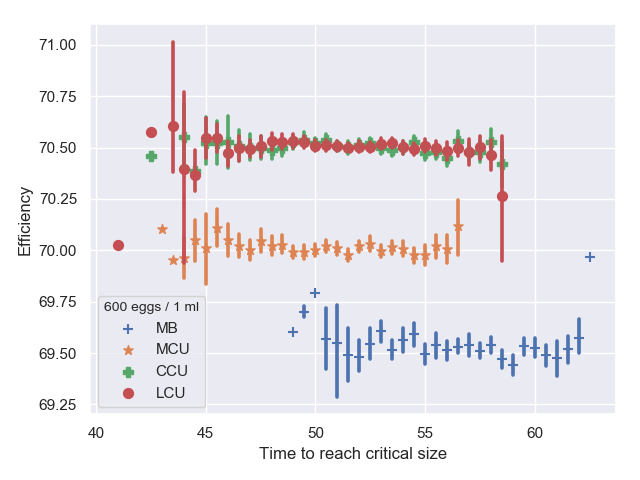
\includegraphics[width=.5\textwidth]{C6/Figs/devt_dist/alive_eff_vs_devt_MCU}
  }
  \subfloat[Mean initial feeding rate distribution]{
  \centering
  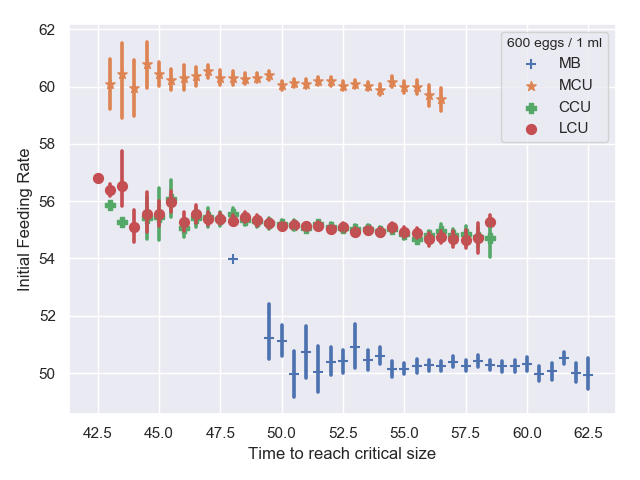
\includegraphics[width=.5\textwidth]{C6/Figs/devt_dist/alive_frc_vs_devt_MCU}
  }\\
  \subfloat[Mean critical size distribution]{
  \centering
  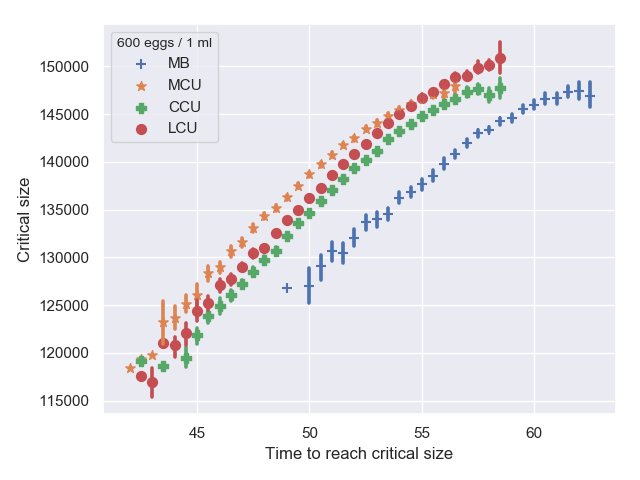
\includegraphics[width=.5\textwidth]{C6/Figs/devt_dist/alive_mc_vs_devt_MCU}
  }
  \subfloat[Mean waste tolerance distribution]{
  \centering
  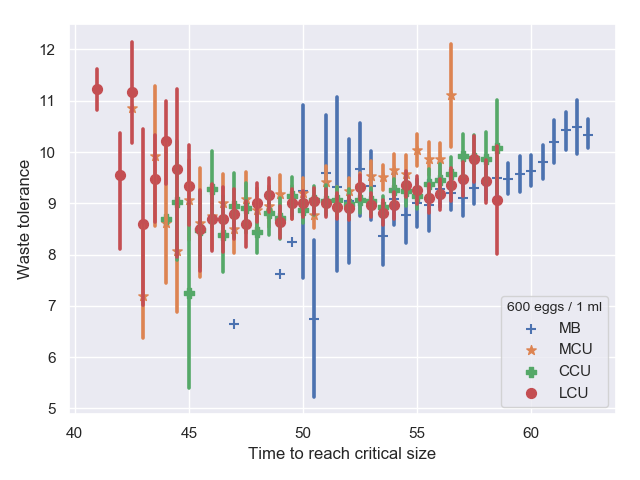
\includegraphics[width=.5\textwidth]{C6/Figs/devt_dist/alive_wt_vs_devt_MCU}
  }
  \caption{Mean trait value distribution of MB, MCU, CCU and LCU populations in 600 eggs / 1.5 ml density at $50^{th}$ generation (errorbars represent 95\% CI)}
  \label{fig:lh_mcu_culture}
\end{figure}
\begin{figure}[p]
  \subfloat[Mean body size distribution]{
  \centering
  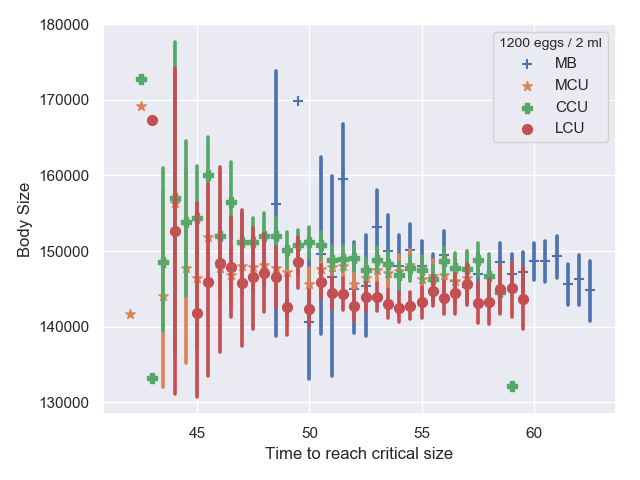
\includegraphics[width=.5\textwidth]{C6/Figs/devt_dist/alive_size_vs_devt_CCU}
  }
  \subfloat[Mean final feeding rate distribution]{
  \centering
  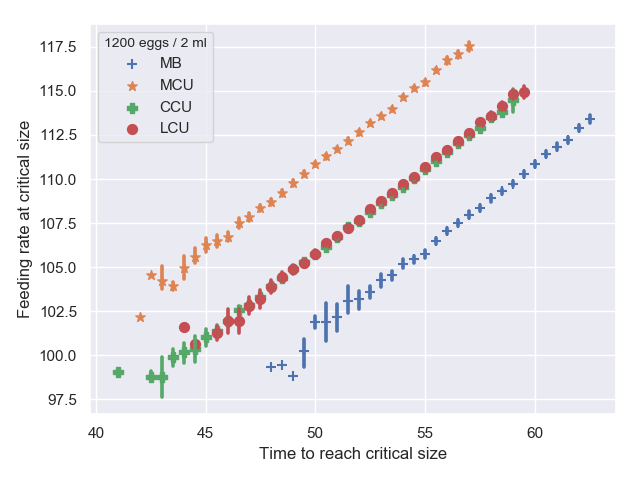
\includegraphics[width=.5\textwidth]{C6/Figs/devt_dist/alive_frt_vs_devt_CCU}
  }\\
  \subfloat[Mean efficiency distribution]{
  \centering
  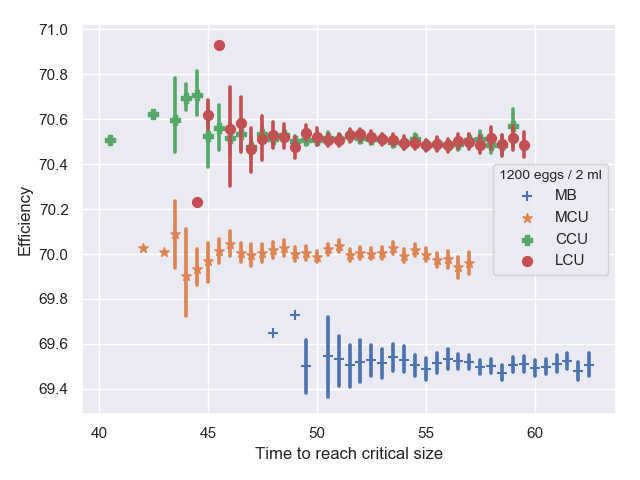
\includegraphics[width=.5\textwidth]{C6/Figs/devt_dist/alive_eff_vs_devt_CCU}
  }
  \subfloat[Mean initial feeding rate distribution]{
  \centering
  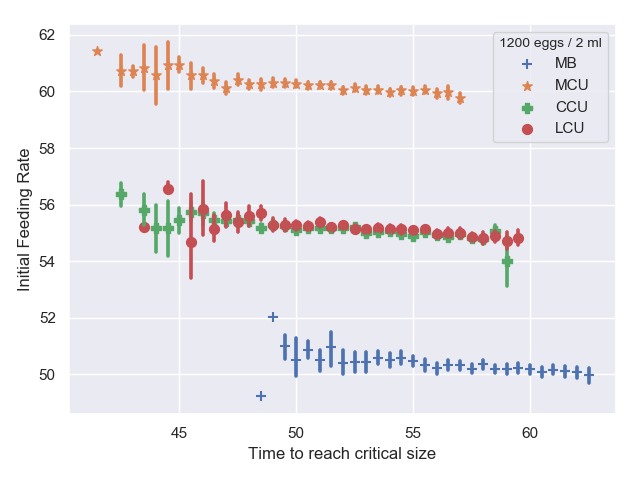
\includegraphics[width=.5\textwidth]{C6/Figs/devt_dist/alive_frc_vs_devt_CCU}
  }\\
  \subfloat[Mean critical size distribution]{
  \centering
  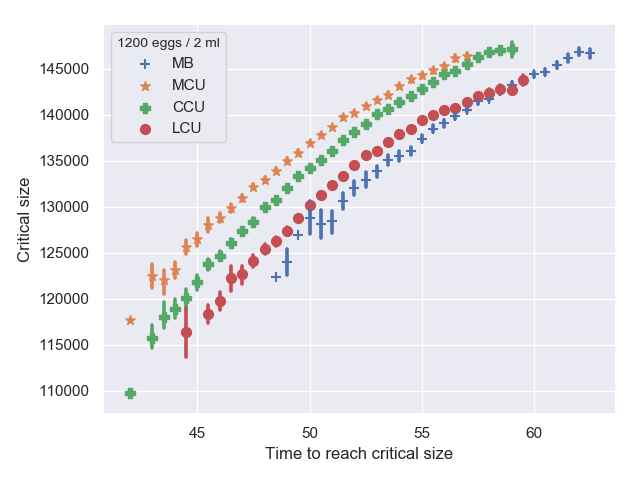
\includegraphics[width=.5\textwidth]{C6/Figs/devt_dist/alive_mc_vs_devt_CCU}
  }
  \subfloat[Mean waste tolerance distribution]{
  \centering
  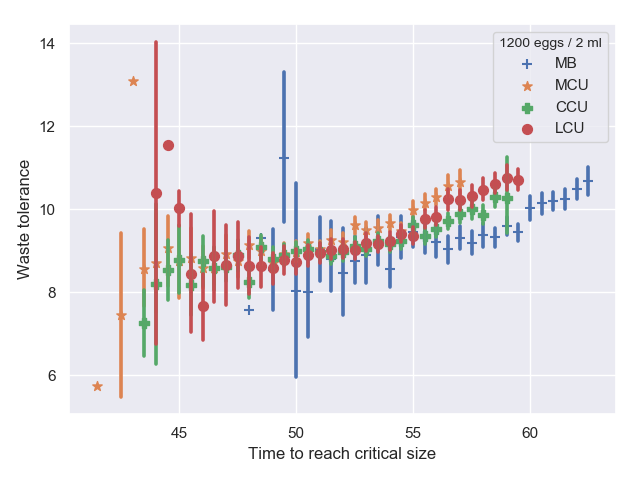
\includegraphics[width=.5\textwidth]{C6/Figs/devt_dist/alive_wt_vs_devt_CCU}
  }
  \caption{Mean trait value distribution of MB, MCU, CCU and LCU populations in 1200 eggs / 3 ml density at $50^{th}$ generation (errorbars represent 95\% CI)}
  \label{fig:lh_ccu_culture}
\end{figure}
\begin{figure}[p]
  \subfloat[Mean body size distribution]{
  \centering
  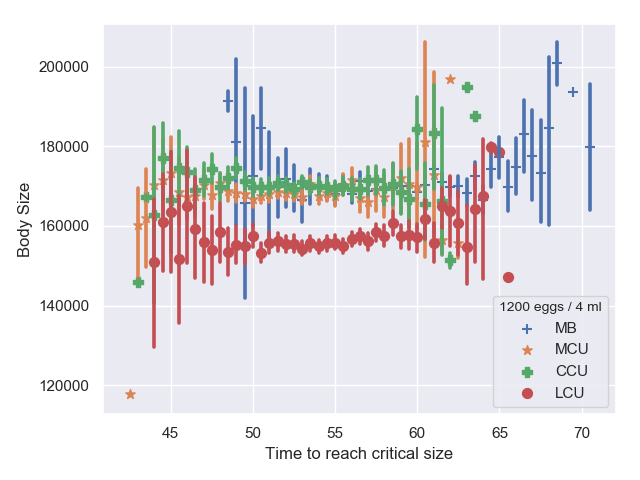
\includegraphics[width=.5\textwidth]{C6/Figs/devt_dist/alive_size_vs_devt_LCU}
  }
  \subfloat[Mean final feeding rate distribution]{
  \centering
  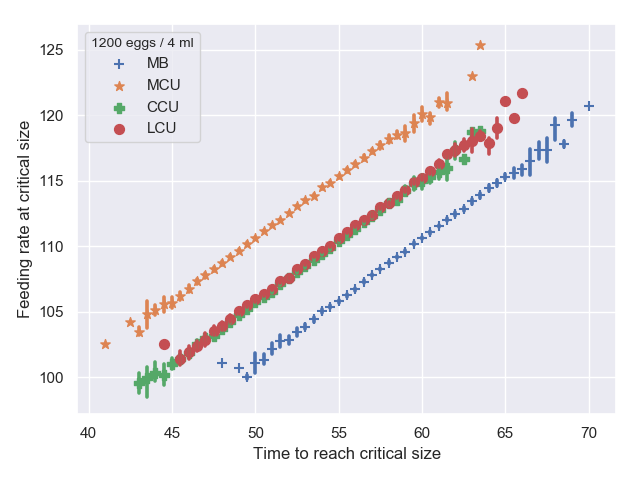
\includegraphics[width=.5\textwidth]{C6/Figs/devt_dist/alive_frt_vs_devt_LCU}
  }\\
  \subfloat[Mean efficiency distribution]{
  \centering
  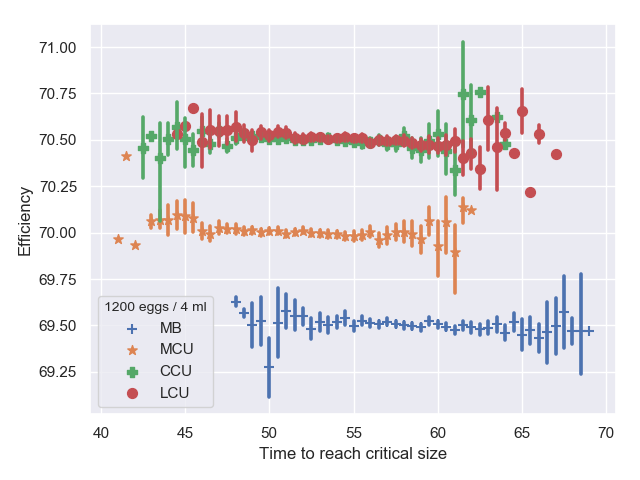
\includegraphics[width=.5\textwidth]{C6/Figs/devt_dist/alive_eff_vs_devt_LCU}
  }
  \subfloat[Mean initial feeding rate distribution]{
  \centering
  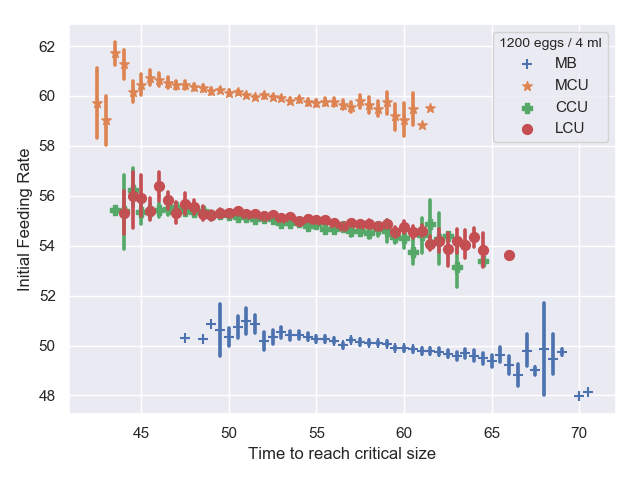
\includegraphics[width=.5\textwidth]{C6/Figs/devt_dist/alive_frc_vs_devt_LCU}
  }\\
  \subfloat[Mean critical size distribution]{
  \centering
  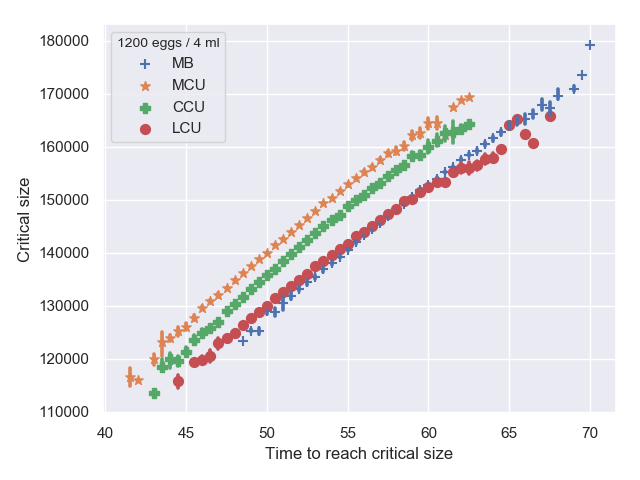
\includegraphics[width=.5\textwidth]{C6/Figs/devt_dist/alive_mc_vs_devt_LCU}
  }
  \subfloat[Mean waste tolerance distribution]{
  \centering
  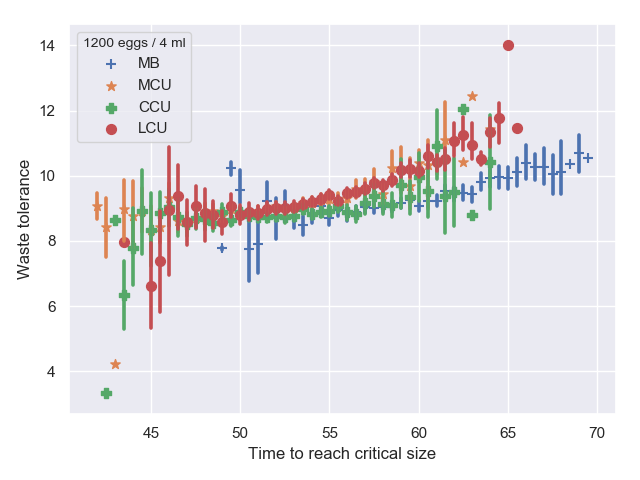
\includegraphics[width=.5\textwidth]{C6/Figs/devt_dist/alive_wt_vs_devt_LCU}
  }
  \caption{Mean trait value distribution of MB, MCU, CCU and LCU populations in 1200 eggs / 6 ml density at $50^{th}$ generation (errorbars represent 95\% CI) }
  \label{fig:lh_lcu_culture}
\end{figure}
\newpage

\section{Effects of Negative Correlation between Feeding Rate and Efficiency}
From the mean trait distribution results, the effect of mean initial feeding rate distribution on body size distribution is clear (fig~\ref{fig:lh_ccu_culture} and fig~\ref{fig:lh_lcu_culture}). If initial feeding rate is negatively correlated with development time, then the model would give a U-shped body size distribution found in the larval crowded populations (ref). To understand further how these correlation between larval competitive traits would affect other life-history traits, I considered a negative correlation between initial feeding rate and efficiency in my model. Efficiency is derived at each generation from the distribution of initial feeding rate. It is given as:
\[\epsilon_{i} = K_{\epsilon} - x_{6}*fr_{i}\]
Here,
$\epsilon_{i}$: efficiency of $i^{th}$ larva;\\
$fr_{i}$: initial feeding rate of $i^{th}$ larva;\\
$x_{6}$: scaling parameter;\\
$K_{\epsilon}$: Maximum value of efficiency (constant).\\\\
Using this correlation, timeseries was run for initial conditions given in table (no.) and same simulations as previous section were performed (replicate=5). The resluts show negative correlation of initial feeding rate across all populations at all four densities (see fig~\ref{fig:neg_corr_frc}). Due to forced negative correlation between initial feeding rate and efficiency, mean efficiency distribution shows that late developing ones have higher efficiency (see fig~\ref{fig:neg_corr_eff}). Fig~\ref{fig:neg_corr_frt} shows that final feeding rate is higher for late developing larvae even if there efficiency is higher and initial feeding rate is lower across all populations at all densities. Fig~\ref{fig:neg_corr_bs} was plotted with higher replicates (n=15) to obtain a clear visualization. Here MCU, CCU and LCU population have mean body size first decreasing then inreasing and decreasing variation wrt development time in MB and CCU culture. Such pattern is not visible in MB and LCU culture.
\begin{figure}[p]
  \subfloat[60 eggs / 6 ml]{
  \centering
  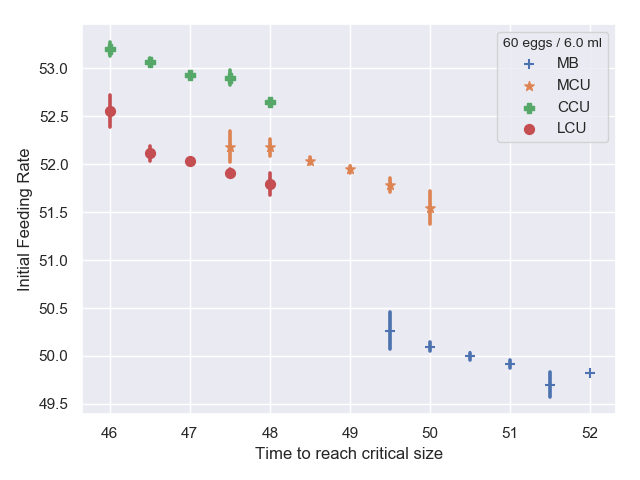
\includegraphics[width=.5\textwidth]{C6/Figs/neg_corr/neg_alive_frc_vs_devt_MB}
  }
  \subfloat[600 eggs / 1.5 ml]{
  \centering
  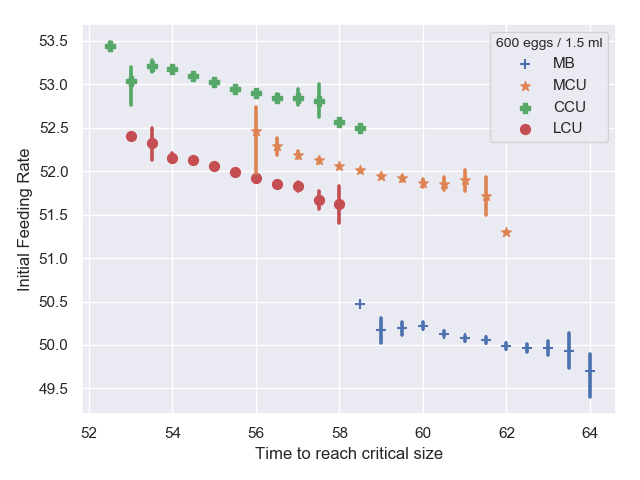
\includegraphics[width=.5\textwidth]{C6/Figs/neg_corr/neg_alive_frc_vs_devt_MCU}
  }\\
  \subfloat[1200 eggs / 3 ml]{
  \centering
  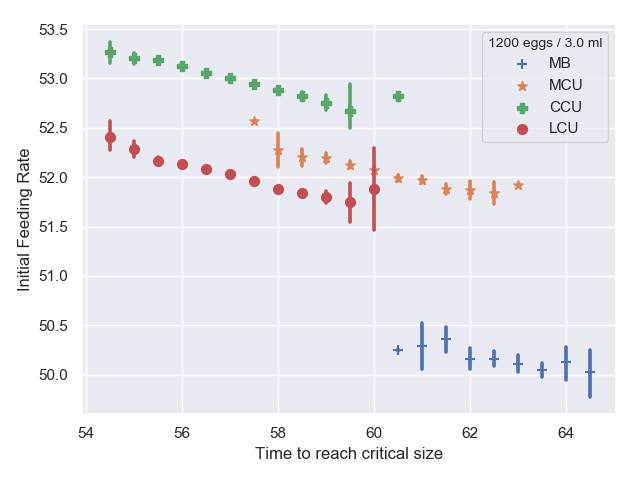
\includegraphics[width=.5\textwidth]{C6/Figs/neg_corr/neg_alive_frc_vs_devt_CCU}
  }
  \subfloat[1200 eggs / 6 ml]{
  \centering
  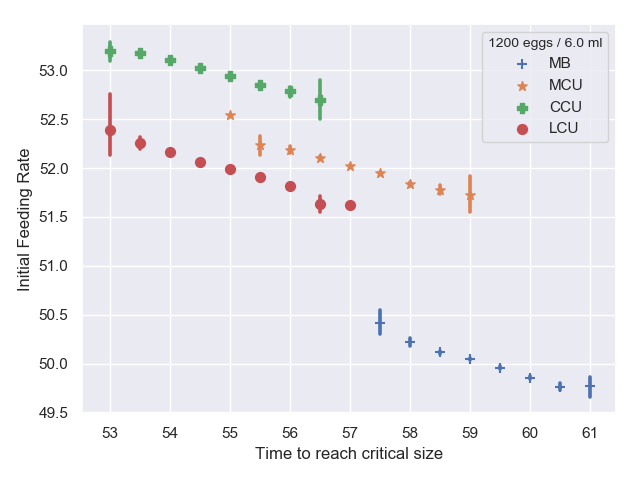
\includegraphics[width=.5\textwidth]{C6/Figs/neg_corr/neg_alive_frc_vs_devt_LCU}
  }
  \caption{Mean initial feeding rate distribution of MB, MCU, CCU and LCU populations in (a) 60 eggs / 6 ml, (b) 600 eggs / 1.5 ml, (c) 1200 eggs / 3 ml and (d) 1200 eggs / 6 ml densities (errorbars represent 95\% CI)}
  \label{fig:neg_corr_frc}
\end{figure}
\begin{figure}[p]
  \subfloat[60 eggs / 6 ml]{
  \centering
  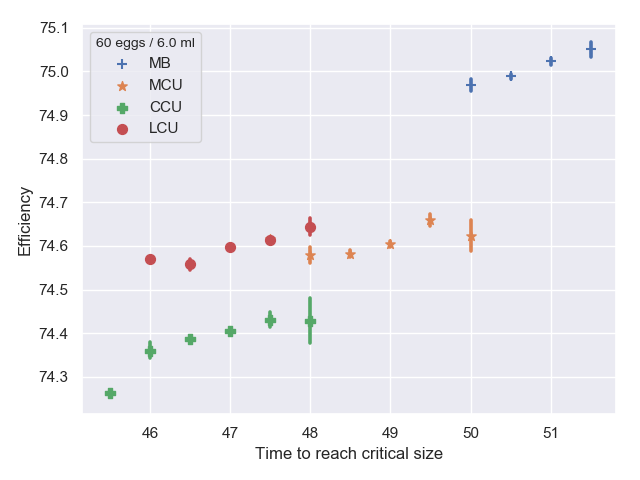
\includegraphics[width=.5\textwidth]{C6/Figs/neg_corr/neg_alive_eff_vs_devt_MB}
  }
  \subfloat[600 eggs / 1.5 ml]{
  \centering
  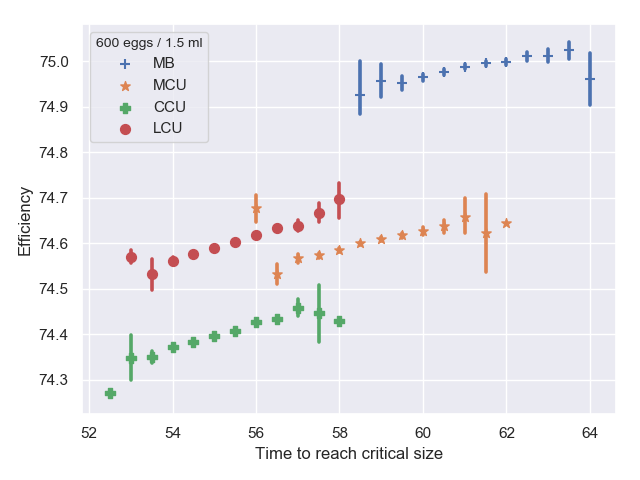
\includegraphics[width=.5\textwidth]{C6/Figs/neg_corr/neg_alive_eff_vs_devt_MCU}
  }\\
  \subfloat[1200 eggs / 3 ml]{
  \centering
  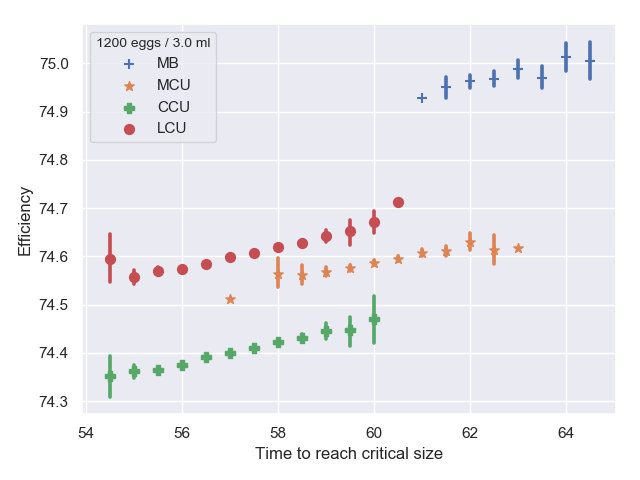
\includegraphics[width=.5\textwidth]{C6/Figs/neg_corr/neg_alive_eff_vs_devt_CCU}
  }
  \subfloat[1200 eggs / 6 ml]{
  \centering
  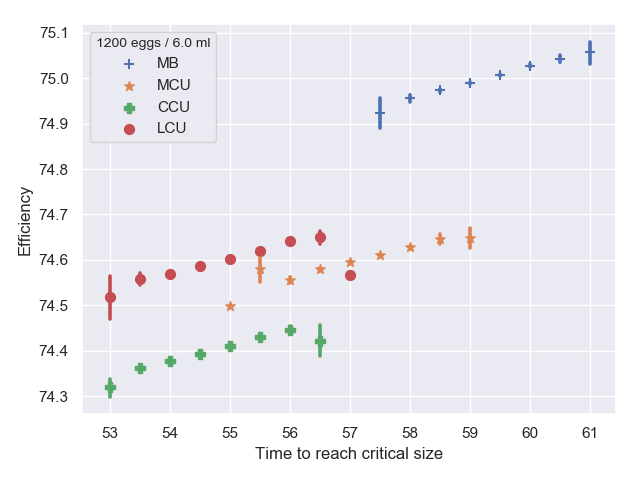
\includegraphics[width=.5\textwidth]{C6/Figs/neg_corr/neg_alive_eff_vs_devt_LCU}
  }
  \caption{Mean efficiency distribution of MB, MCU, CCU and LCU populations in (a) 60 eggs / 6 ml, (b) 600 eggs / 1.5 ml, (c) 1200 eggs / 3 ml and (d) 1200 eggs / 6 ml densities (errorbars represent 95\% CI)}
  \label{fig:neg_corr_eff}
\end{figure}
\begin{figure}[p]
  \subfloat[60 eggs / 6 ml]{
  \centering
  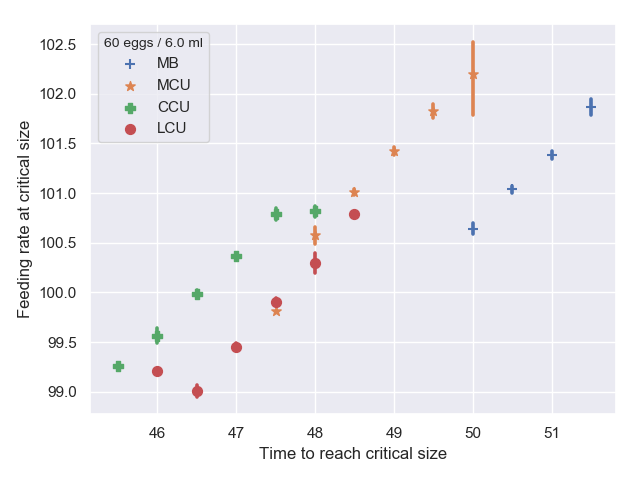
\includegraphics[width=.5\textwidth]{C6/Figs/neg_corr/neg_alive_frt_vs_devt_MB}
  }
  \subfloat[600 eggs / 1.5 ml]{
  \centering
  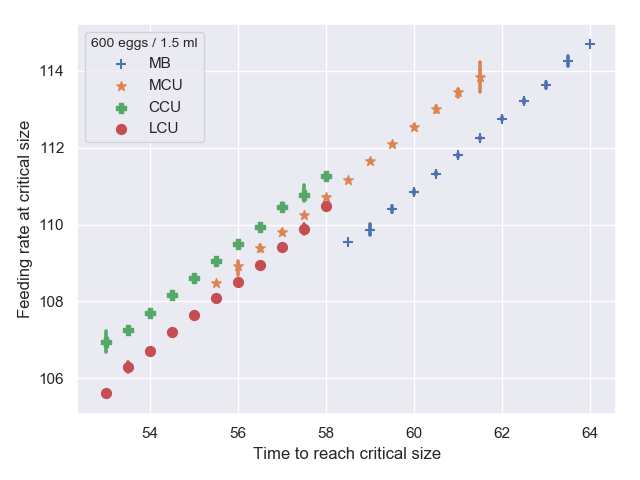
\includegraphics[width=.5\textwidth]{C6/Figs/neg_corr/neg_alive_frt_vs_devt_MCU}
  }\\
  \subfloat[1200 eggs / 3 ml]{
  \centering
  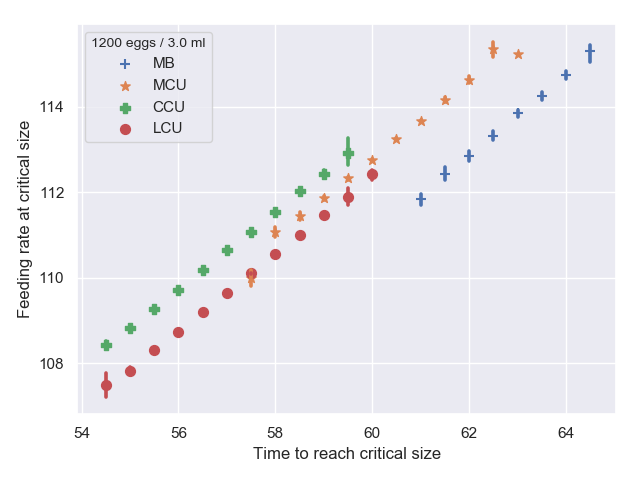
\includegraphics[width=.5\textwidth]{C6/Figs/neg_corr/neg_alive_frt_vs_devt_CCU}
  }
  \subfloat[1200 eggs / 6 ml]{
  \centering
  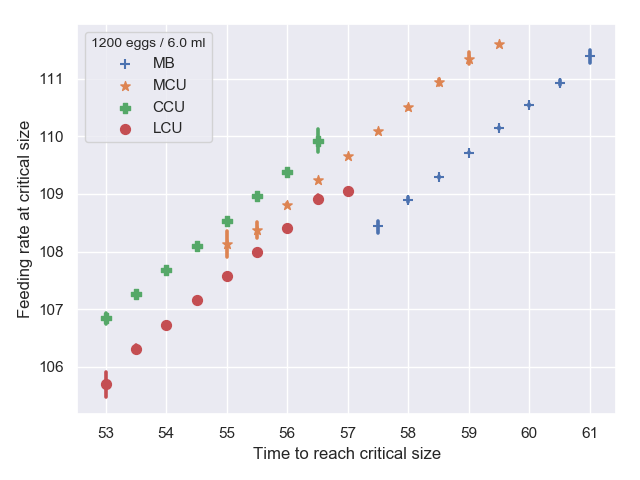
\includegraphics[width=.5\textwidth]{C6/Figs/neg_corr/neg_alive_frt_vs_devt_LCU}
  }
  \caption{Mean feeding rate at critical size of MB, MCU, CCU and LCU populations in (a) 60 eggs / 6 ml, (b) 600 eggs / 1.5 ml, (c) 1200 eggs / 3 ml and (d) 1200 eggs / 6 ml densities (errorbars represent 95\% CI)}
  \label{fig:neg_corr_frt}
\end{figure}
\begin{figure}[p]
  \subfloat[60 eggs / 6 ml]{
  \centering
  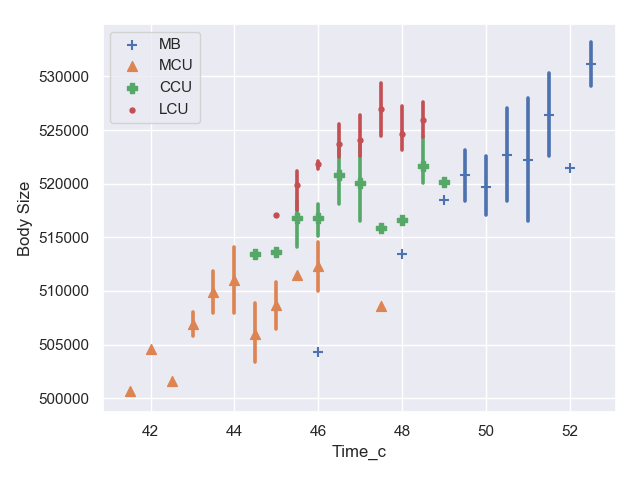
\includegraphics[width=.5\textwidth]{C6/Figs/neg_corr/neg_alive_size_vs_devt_MB}
  }
  \subfloat[600 eggs / 1.5 ml]{
  \centering
  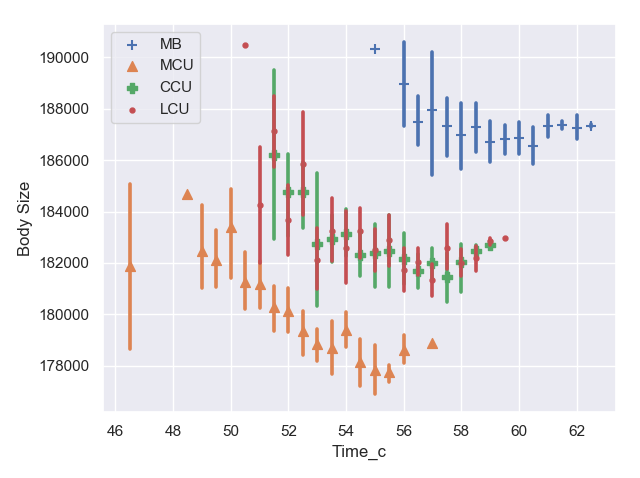
\includegraphics[width=.5\textwidth]{C6/Figs/neg_corr/neg_alive_size_vs_devt_MCU}
  }\\
  \subfloat[1200 eggs / 3 ml]{
  \centering
  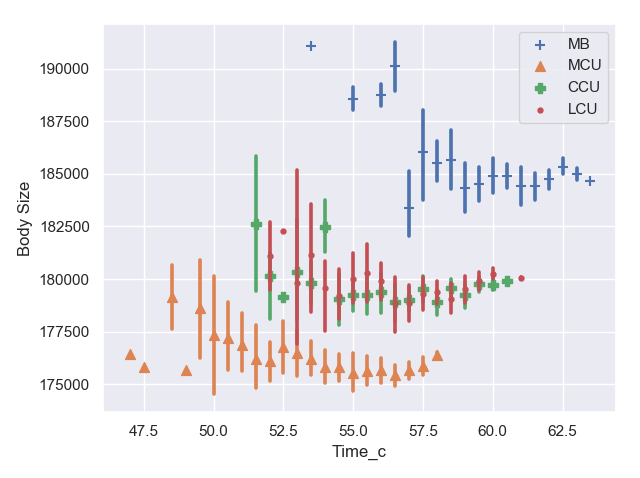
\includegraphics[width=.5\textwidth]{C6/Figs/neg_corr/neg_alive_size_vs_devt_CCU}
  }
  \subfloat[1200 eggs / 6 ml]{
  \centering
  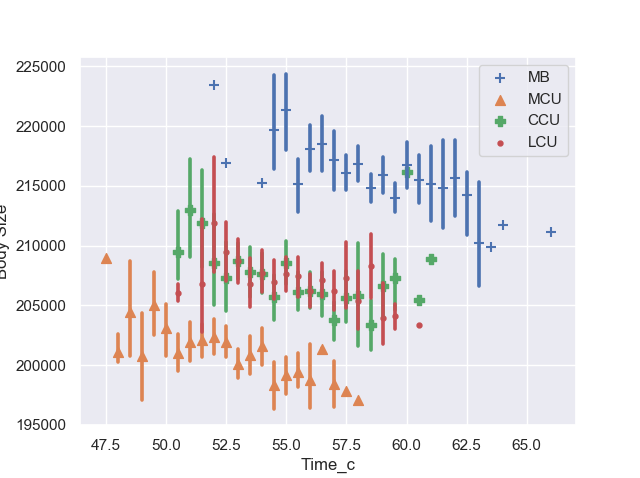
\includegraphics[width=.5\textwidth]{C6/Figs/neg_corr/neg_alive_size_vs_devt_LCU}
  }
  \caption{Mean efficiency distribution of MB, MCU, CCU and LCU populations in (a) 60 eggs / 6 ml, (b) 600 eggs / 1.5 ml, (c) 1200 eggs / 3 ml and (d) 1200 eggs / 6 ml densities (errorbars represent 95\% CI)}
  \label{fig:neg_corr_bs}
\end{figure}
\pagebreak
